\documentclass[12pt]{article}
\usepackage{a4wide}
\usepackage{latexsym}
\usepackage{amssymb}
\usepackage{epic}
\usepackage{graphicx}
\usepackage{comment}
\usepackage{graphicx}
%\pagestyle{empty}
\newcommand{\tr}{\mbox{\sf true}}
\newcommand{\fa}{\mbox{\sf false}}
\newcommand{\bimp}{\leftrightarrow}

\begin{document}
\section*{Automated Reasoning\\Assignment 1}

\begin{center}
Wouter Geraedts (s0814857) \\
Judith van Stegeren (s3014827)\\
\end{center}

\vspace{8mm}

\subsection*{Trucks and pallets}
The problem: find a way to load pallets of different objects onto 6 trucks, while adhering to various constraints. 
Investigate the maximum number of pallets of prittles that can be delivered, 
and show how for that number all pallets may be divided over the six trucks.

We have generalized the problem in the following way: given $t$ trucks with a capacity of $c$ that can carry at most $p$ pallets, an array \texttt{amount} of numbers of pallets of nuzzles, skipples, crottles and dupples and an array \texttt{weight} of the weight of a pallet of each of these items, maximize the number of pallets of prittles that can be delivered.
Note that throughout the text we use the number `$0$' (the index corresponding to nuzzles), the full object name `\texttt{nuzzles}' or the single letter `\texttt{n}' interchangably, to increase readability.

We start out by introducing our representation. We have a function 
\[\texttt{Pallets :: Int -> Int -> Int}\]
\texttt{Pallets t o} returns the number of pallets of object \texttt{o} that truck \texttt{t} is carrying.

Trucks cannot carry a negative amount of pallets:
\[ \bigwedge_{0 \le \texttt{i} < t} \bigwedge_{0 \le \texttt{j} < o} \texttt{Pallets i j} \ge 0 \]

Trucks cannot carry more than $p$ pallets:
\[ \bigwedge_{0 \le \texttt{i} < t} ~ ( \sum_{0 \le \texttt{j} < o} \texttt{Pallets i j} ) \le p \]

Each pallet of object \texttt{o} weighs \texttt{weight[o]} kg. Trucks cannot carry more than the maximum weight of $c$ kg:
\[ \bigwedge_{0 \le \texttt{i} < t} ~ (\sum_{0 \le \texttt{j} < o} \texttt{Pallets i j} \cdot \texttt{weight[j]}) \le c \]
Prittles and crottles are not allowed in the same truck. In other words, for every truck \texttt{t} it should not be possible that \texttt{(Pallets t prittles)} and \texttt{(Pallets t crottles)} are both greater than 0:
\[ \bigwedge_{0 \le \texttt{i} < t} \neg \left(( \texttt{Pallets i prittles} > 0) \wedge (\texttt{Pallets i crottles} > 0 )\right)\]

There can be at most 2 trucks carrying skipples. To be able to express this constraint, we first need to count the number of trucks carrying skipples. We introduce a variable \texttt{skt} to count the number of skipple-carrying trucks. We calculate the value of this integer by summing over all trucks \texttt{t} with a simple if-then-else-statement in yices: 
\[ \texttt{skt} = \sum_{0\le \texttt{i} < t} \texttt{(ite (> (Pallets i skipples) 0) 1 0)}\]

Now we can easily express the constraint by adding the following to our formula:
\[ \texttt{skt} \le 2 \]

We have to deliver \texttt{amount[o]} pallets of object \texttt{o}. Finally we assert that all pallets in the delivery should be loaded onto the trucks:

\[ \bigwedge_{0 \le \texttt{i} < o} \sum_{0 \le \texttt{j} < t} \texttt{Pallets j o} = \texttt{amount[o]}\]

We fill in a number for \texttt{amount[prittles]} and see if the formule is satisfiable. We use binary search to find the maximum number of pallets of prittles that we can deliver.
The formula was satisfiable when \texttt{amount[prittles]} was equal to 20.
We show the assignment found by the solver in figure \ref{fig:sub1table}.
Since this brings the total amount of delivered pallets to 47 and the maximum number of pallets we can carry with the six trucks is 48, this seems like a plausible solution.

\begin{figure}[h]
    \begin{center}
        \begin{tabular}{r|ccccc}
        truck & \texttt{n} & \texttt{p} & \texttt{s} & \texttt{c} & \texttt{d} \\\hline
        $t_0$ & 1 & 0 & 7 & 0 & 0 \\
        $t_1$ & 0 & 0 & 0 & 5 & 2 \\
        $t_2$ & 2 & 6 & 0 & 0 & 0 \\
        $t_3$ & 0 & 0 & 0 & 5 & 3 \\
        $t_4$ & 0 & 8 & 0 & 0 & 0 \\
        $t_5$ & 1 & 6 & 1 & 0 & 0 \\\hline
        total & 4 & 20 & 8 & 10 & 5 \\
        \end{tabular}
    \end{center}
    \caption{Assignment of pallets to trucks for an optimal solution.}
    \label{fig:sub1table}
\end{figure}

\subsection*{Scheduling of jobs}
The problem: schedule twelve jobs with different running times, while adhering to a list of constraints.
Investigate the minimal running time needed to complete all jobs.
Our solution works for a arbitrary number of jobs.
We want to schedule $j$ jobs numbered from 1 to $j$.
The running time for job $i$ is $rt_i = i+5$.

Our representation is as follows.
We have a timeline of length $T$.
For every moment in time, we have a status code for every job: it is either ready (0), running (1) or finished (2). 
For this we have the function 
\[\texttt{Status :: Int -> Int -> Int}\]
\texttt{Status 1 10 2} means that job 1 at timeframe 10 is finished. 

The job status must be either 0, 1 or 2, for all jobs and moments in time:
\[ \bigwedge_{0 \le \texttt{t} < T} ~ \bigwedge_{0 \le \texttt{i} < j} \texttt{Status i t} \ge 0\wedge \texttt{Status i t} \le 2\]

We now want to specify the correct behaviour for each job. 
Since the running time for each job $i$ is $rt_i$ and we want it to be finished before or on timeframe $T-1$ (the end of the timeline), we have to start job $i$ at timeframe $T - rt_i$ at the latest.
We take $st_i$ as the starting time of job $i$, with $0 \le st_i < lt_i$ and $lt_i = T-rt_i$.

Before a job starts (1), it must be ready (0):
\[ \bigwedge_{0 \le \texttt{tt} < st_i} \texttt{Status i tt} = 0 \]

We want the jobs to run without interrupt.
In other words, if a job has started, it will not stop until it is finished. 
If job $i$ starts at timeframe $st_i$, it keeps running in timeframes $st_i \dots (st_i + rt_i)$.
\[ \bigwedge_{0 \le \texttt{rt} < rt_i} \texttt{Status i (st+rt)} = 1 \]

If the job is done running, it is finished and it will stay finished for the remainder of the timeframes, starting at timeframe $st_i + rt_i$.
\[ \bigwedge_{0 \le \texttt{tt} < T-st-rt_i} \texttt{Status i tt} = 2 \]

If we put these three conditions together, we get:
\[ \begin{array}{rll}
    \bigwedge_{0 \le \texttt{i} < j} \bigvee_{0 \le \texttt{st} < lt_i} \left( \right.&& \\
    & \bigwedge_{0 \le \texttt{tt} < st} & \texttt{Status i tt} = 0 ~ \wedge \\
    & \bigwedge_{0 \le \texttt{tt} < rt_i} & \texttt{Status i st+tt} = 1 ~ \wedge \\
    & \bigwedge_{0 \le \texttt{tt} < T-st-rt_i} & \texttt{Status i tt} = 2 \\
\left. \right)
\end{array} \]

Now we have a number of job specific constraints. 
If we want to express that job a is only allowed to start if job b and c have finished, we write: 
\[ \bigwedge_{0 \le \texttt{tt} < T} (\texttt{Status a tt} = 1) \rightarrow (\texttt{Status b tt} = 2 \wedge \texttt{Status c tt} = 2) \]

Job 3 may only start if job 1 and 2 have finished.
\[ \bigwedge_{0 \le \texttt{tt} < T} (\texttt{Status 3 tt} = 1) \rightarrow (\texttt{Status 1 tt} = 2 \wedge \texttt{Status 2 tt} = 2) \]
Job 5 may only start if job 3 and 4 have finished.
\[ \bigwedge_{0 \le \texttt{tt} < T} (\texttt{Status 5 tt} = 1) \rightarrow (\texttt{Status 3 tt} = 2 \wedge \texttt{Status 4 tt} = 2) \]
Job 7 may only start if job 3, 4 and 6 have finished.
\[ \bigwedge_{0 \le \texttt{tt} < T} (\texttt{Status 7 tt} = 1) \rightarrow (\texttt{Status 3 tt} = 2 \wedge \texttt{Status 4 tt} = 2 \wedge \texttt{Status 6 tt} = 2) \]
Job 9 may only start if job 5 and 8 have finished.
\[ \bigwedge_{0 \le \texttt{tt} < T} (\texttt{Status 9 tt} = 1) \rightarrow (\texttt{Status 5 tt} = 2 \wedge \texttt{Status 8 tt} = 2) \]
Job 11 may only start if job 10 has finished.
\[ \bigwedge_{0 \le \texttt{tt} < T} (\texttt{Status 11 tt} = 1) \rightarrow (\texttt{Status 10 tt} = 2\]
Job 12 may only start if job 9 and 11 have finished.
\[ \bigwedge_{0 \le \texttt{tt} < T} (\texttt{Status 12 tt} = 1) \rightarrow (\texttt{Status 9 tt} = 2 \wedge \texttt{Status 11 tt} = 2) \]

Another constraint is that job 8 may not start earlier than job 5, in other words, we want that if job 5 starts running, job 8 is either running as well or already finished:
\[ \bigwedge_{0 \le \texttt{tt} < T} (\texttt{Status 5 tt} = 1) \rightarrow (\texttt{Status 8 tt} > 0) \]

For job 5, 7 and 10 we have that no two of these job may be running at the same time. 
We introduce a variable $nr_t$ to count the number of running jobs 5, 7 and 10 in timeframe $t$.
We calculate the value of this integer by summing over jobs 5, 7 and 10 with a simple if-then-else-statement in yices: 
\[ nr_t = \sum_{i \in \{5,7,10\}} \texttt{ite (= 1 (Status i t)) 1 0} \]
Now we can enforce the constraint by counting the number of running jobs 5, 7 and 10 in each timeframe, 
and stating that this number is not allowed to be greater than 1. 
\[ \bigwedge_{0 \le t < T} nr_t \le 1\]

We filled in a value for the variable time (the length of the timeline) 
and asked the SMT-solver whether the formule was satisfiable. 
We used binary search to find the minimal number of time frames needed to schedule all jobs. 
We found the value 59. 
Below is a Gant chart that shows us how the jobs were scheduled within 59 time frames:
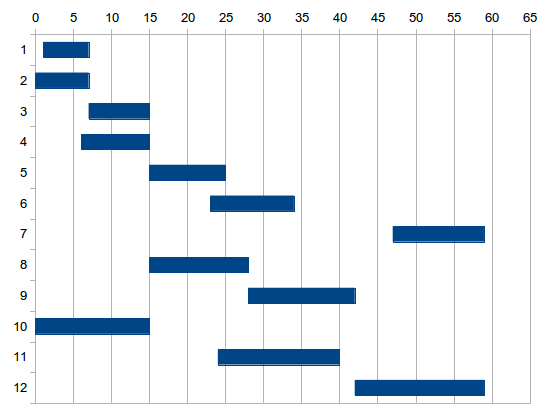
\includegraphics[width=15cm]{gantchart.png}

\subsection*{Computation steps}
The problem: given a set of $N$ variables $a_1, \cdots, a_N$ and their initial value.
For all variables except $a_1$ and $a_N$, it is possible to either do nothing, or assign a new value to the variable:
\[ a_v = a_{v-1} + a_{v+1} \]
We need to find the minimum number of steps required for any of these variables to attain the value 157.
We compute this by fixing the number of steps $T$, and then defining a function
\[\texttt{A :: Int -> Int -> Int}\]
such that \texttt{A v t} is the value of variable $a_v$ after $t$ steps.

First we define the initial value for all variables:
\[ \bigwedge_{1 \le \texttt{v} \le N} \texttt{A v 0} = \texttt{v} \]
Then we define the steps allowed for each variable.
The $t^\mathtt{th}$ step can be done by precisely one variable $a_v$ in $\{ a_2, \cdots, a_{N-1} \}$.
This step is done by updating this variable:
\[\texttt{A v (t+1)} = \texttt{A (v-1) t} + \texttt{A (v+1) t}\]
And all other variables must remain unchanged:
\[\bigwedge_{ \texttt{u} \in \{1, \cdots, N\} \setminus \{ \texttt{v} \} } \texttt{A u (t+1)} = \texttt{A u t}\]

This can be done for any step $t$, thus this entire section can be written down with:
\[
    \bigwedge_{0 \le \texttt{t} < T}
    \bigvee_{1 < \texttt{v} < N}
        \left (\texttt{A v (t+1)} = \texttt{A (v-1) t} + \texttt{A (v+1) t} \right)
        ~\wedge~
        \left( \bigwedge_{ \texttt{u} \in \{1, \cdots, N\} \setminus \{ \texttt{v} \} } \texttt{A u (t+1)} = \texttt{A u t} \right)
\]

Finally we define the end-goal:
\[ \bigvee_{1 \le \texttt{v} \le N} \texttt{A v T} = 157 \]

To find the minimum number of steps required, we use binary search on the number of steps $T$.
If for any $T$ the problem is satisfiable, the problem is also satisfiable for $T+1$, because the ``do nothing''-step can always be chosen.
Thus binary search is applicable in this case.

Our algorithm for binary search concludes that the problem can be solved in at least 10 steps.

\end{document}
